%input "worldcup.bib"

\documentclass[letterpaper,nocopyrightspace]{sig-alternate}
%\documentclass[letterpaper,nocopyrightspace]{acm_proc_article-sp}
\sloppy % makes TeX less fussy about line breaking

\usepackage{subfigure}
\usepackage{epsfig}
\usepackage{multirow}

%for PDF features - http://www.ce.cmu.edu/~kijoo/latex2pdf.pdf
\usepackage[pdftex,colorlinks]{hyperref} % For the bookmark/hyperlinks

% style of the figure captions
\newcommand{\capttext}{\protect\centering\em}

\setlength{\pdfpagewidth}{8.5in}
\setlength{\pdfpageheight}{11in}

\hypersetup{%
    pdftitle={Characterising User Interactivity for Sports Video-on-Demand},
    pdfauthor={Andrew Brampton, Andrew MacQuire, Idris A. Rai, Nicholas J. P. Race, Laurent Mathy and Michael Fry},
    pdfkeywords={Interactive, Sports, Video-on-Demand, Worldcup, Content Distribution},
    bookmarksnumbered,
    pdfstartview={FitV},
    linkcolor={black},%: Color for normal internal links.
    anchorcolor={black},%: Color for anchor text.
    citecolor={black},%: Color for bibliographical citations in text.
    filecolor={black},%: Color for URLs which open local files.
    menucolor={black},%: Color for Acrobat menu items.
    pagecolor={black},%: Color for links to other pages
    urlcolor={black}%: Color for linked URLs.
}

\numberofauthors{3}
\author{
\alignauthor Andrew Brampton $\dagger$
\alignauthor Andrew MacQuire  $\dagger$
\alignauthor Idris A. Rai  $\dagger$
\and
\alignauthor Nicholas J.P. Race  $\dagger$
\alignauthor Laurent Mathy  $\dagger$
\alignauthor Michael Fry  $\ddagger$
\end{tabular}\\\tiny~\\
\begin{tabular}{cc}
$\dagger$\normalsize Lancaster University &
\hspace{3em}$\ddagger$\normalsize University of Sydney\hspace{8em} \\
\small\{brampton,macquire,rai,race,laurent\}@comp.lancs.ac.uk &
\hspace{3em}\small michael.fry@usyd.edu.au\hspace{8em} \\
}
\date{}

\begin{document}

\conferenceinfo{NOSSDAV}{'07 Urbana, Illinois USA}
\CopyrightYear{2007}
\crdata{978-1-59593-746-9/06/2007}

\title{Characterising User Interactivity for Sports Video-on-Demand}
\maketitle

\begin{abstract}
This paper presents a detailed characterisation of user behaviour
for a series of interactive sport videos from the 2006 FIFA World
Cup. In addition to generic VCR-like features, our custom-built
Video-on-Demand architecture enabled us to provide advanced
interactivity features such as bookmarking. We illustrate how such
functionality may have a dramatic impact on how users consume
content. A detailed discussion is also provided on how content
distributors may turn this knowledge to their advantage, and thus
increase the efficiency of their delivery networks.
\end{abstract}

\section{Introduction}

In recent years the Internet has increasingly been used to
distribute bandwidth-intensive, low-latency streaming media. Due to
the resources required to deliver such content, dedicated Content
Distribution Networks (CDNs) are often used to improve the
end-user's experience. As such systems evolve, users expect
correspondingly improved interactive functionality; something which
is increasingly difficult to achieve with diverse content types
exhibiting varied access patterns. In order to provide a high
quality of service, modern CDNs must therefore have an in-depth
understanding of user behaviour regarding different content types.

A number of previous papers have already studied the
characterisation of user behaviour for Video-on-Demand (VoD)
content. Some have studied single genres such as educational
videos~\cite{Almeida01Analysis,Chesire01Measurement,Acharya00Characterizing},
whereas others have examined a range of video
types~\cite{Costa04Analyzing,Sripanidkulchai04Analysis,Cherkasova02Characterizing,yu2006uub}.
This paper is closely related to previous work that examined user
characterisation for {\em interactive} video. Similar studies exist
where logs were analysed from VoD systems that support VCR
interactivity, \emph{i.e.} the ability to pause, resume and skip
back and forth within a given video
stream~\cite{Costa04Analyzing,Tang03MediSyn,vilas2005user}. The
typical approach in these studies has been to analyse either
publicly available traces of static content (such as those at the
Internet Traffic Archive~\cite{ITA}), or privately obtained logs of
more dynamic streaming content from larger networks such as
Akamai's~\cite{akamai}.

In this paper, we study user behaviour for an interactive VoD system
that serves users specifically with video from the 2006 FIFA World
Cup. A key distinguishing element of our work is the fact that we
implemented our own VoD system, designed to offer novel interactive
functionality beyond typical VCR-like features. The prime example of
this is \emph{bookmarking}: direct links to points of interest
within the video. Our system also allowed users to contribute their
own bookmarks at any time, distinct from those added during the
publishing process. An example of a bookmark within our content
could be a common event such as the match kick-off, or a potentially
more popular event, such as a goal.

Previous studies making use of entertainment content may have
witnessed the classic start-to-finish playback model in their access
patterns, with occasional user VCR interactivity. In our experiment,
however, sports content proved highly dynamic. Users often chose to
watch (and re-watch) small segments of the full video, in a complete
departure from the start-to-finish model. The behaviour observed may
also be present in other sports, and different content genres
(\emph{e.g.} educational, entertainment, news, \emph{etc.}), as
these genres often have a few popular highlights.

We found that the bookmark functionality in our system had a
significant impact on user behaviour, leading to access patterns
quite dissimilar from previous related work. We identified
distributions, namely {\em log-normal}, {\em Weibull} and {\em
normal}, to best model various metrics and workload properties.
These models can be used to drive simulations of the type of
interactivity behaviour studied in this paper. We also discuss how
delivery networks can exploit the observed behaviour to improve
user-perceived performance. For instance, we show that the order in
which users view bookmarks can be predicted based on previous
activity, enabling CDNs to leverage this data for performance gains.

% AM: check following any structural changes

The remainder of this paper is structured as follows:
Section~\ref{sect:methodology} describes our experimental setup,
while Section~\ref{sect:results} analyses the results.
Section~\ref{sect:conclusion} concludes the paper with a discussion
of the impact of our results on existing Content Distribution
Networks.

\section{Experimental Setup}
\label{sect:methodology}
\begin{figure}[tb]
\centering
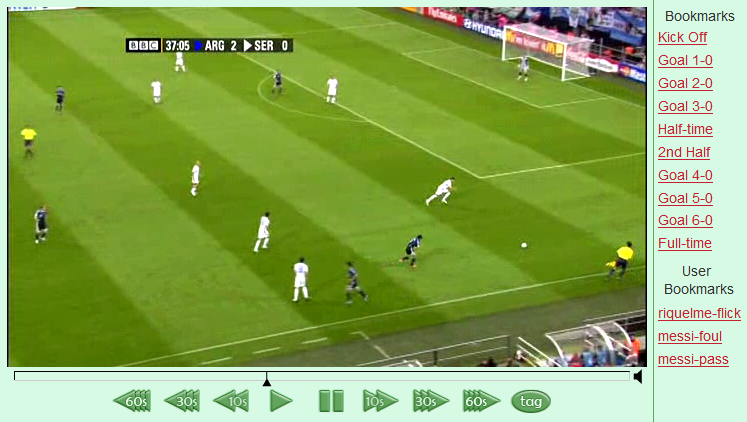
\epsfig{file=./diagrams/InterfaceEdit.png,width=0.45\textwidth}
\caption{\capttext Video-On-Demand Interface}
\label{fig:server_setup}
\end{figure}

We set up a simple, interactive video-on-demand
system. The system was divided
into three main components: the capture server, the Video-on-Demand
server, and a web interface~\footnote{More information about the system and its source
code is available at http://www.rcdn.org/}.

% The capture server

Our capture server recorded public broadcasts of raw MPEG-2 streams
from the beginning of the pre-match commentary through to the end of
coverage. Once a full match was captured, the system transcoded the
stream to high and low bitrate Macromedia Flash 7 FLV streams (1
Mbps and 300 Kbps respectively). Administrators would then manually
add metadata to the system describing the location of key events
within the match. These locations are referred to as
\emph{bookmarks}, and typically included events such as the
beginning and end of the match, any goals, and other important
events such as red cards. The final FLV streams were then
transferred to the VoD server. This full process typically took 6
hours and thus the matches were available shortly after being
played.

% VoD Server
The VoD system was an Apache webserver, which served the Flash based
user interface over HTTP. This server was only accessible to staff
and students within Lancaster University's campus, and those
connecting remotely via VPN. To aid in logging, the user interface
would make its HTTP requests as verbose as possible, allowing us to
later track users through multiple sessions and determine exactly
which controls were pressed and when. Additionally, each playback
window would maintain a periodic HTTP-request heartbeat with the
server, which was used to determine when connectivity was
unexpectedly lost.

% Web interface
The web interface consisted of two main sections; firstly a index
page allowing the user to select any available match from the World
Cup, and secondly the player interface that displayed the video of
the matches, as shown in Fig.~\ref{fig:server_setup}. The player
interface offered some simple controls to seek around the match. We
were aware that the user interface would constrain the user's
actions, and it was therefore designed to be as simple and generic
as possible. Forward and backward buttons were provided that allowed
seeking 10, 30 and 60 seconds in either direction. These only
accounted for rather small jumps, and so we also provided a seek bar
which enabled users to make potentially large jumps to any
arbitrarily chosen time. Finally, users had the list of
administrator-added \emph{bookmarks} which enabled them to seek
directly to key events. This interface was also extended to allow
users to submit their own bookmarks (via the \emph{tag} button),
which other users could see and select. These user bookmarks covered
events that were not typically bookmarked, but were of particular
interest (such as events that came under later scrutiny).

~\\

\section{Analysis}
\label{sect:results}

The 2006 FIFA World Cup ran from the $9^{th}$ of June until the
$9^{th}$ of July, whereas the results analysed in this paper were
recorded from the $13^{th}$ of June until the $16^{th}$ of July. The
data for the first 4 days was discarded due to alterations made to
the logging system and user interface in that period. Also, the 7
extra days considered after the end of the World Cup were added due
to continued use of the site. A total of 66 matches were logged (64
from the event, and 2 pre-competition friendlies), with 405 unique
users over the one month period. On average 30.7 unique users viewed
each match.

In this section, we use the logs from our experiment to characterise
user properties for our system. {\em R-Square} fitting is used to
determine models for the various features analysed, such as
\emph{popularity}, \emph{session length}, \emph{inter-seek times},
and \emph{bookmark requests}.

\subsection{Interactions}
\label{sect:interactions}

\begin{table}[tb]
\centering {\tiny
\begin{tabular}{|c|c|c|c|}
  \hline
  Action & Occurrences & Percentage(\%) & per Session\\
  \hline

  Back 10s        & 1353 & 5.98  & 0.58 \\
  Back 30s        & 556  & 2.46  & 0.24 \\
  Back 60s        & 775  & 3.43  & 0.33 \\
  Forward 10s     & 3319 & 14.67 & 1.42 \\
  Forward 30s     & 1664 & 7.36  & 0.71 \\
  Forward 60s     & 3488 & 15.42 & 1.49 \\
  Seek-bar        & 2101 & 9.29  & 0.90 \\
  Bookmarks       & 5203 & 23.00 & 2.22 \\
  User bookmarks  & 585  & 2.59  & 0.25 \\
  Add bookmark    & 43   & 0.19  & 0.02 \\
  Pause           & 1847 & 8.16  & 0.79 \\ % There was 103 "double" pauses
  Resume          & 1690 & 7.47  & 0.72 \\ % There was 866 resumes pressed needlessly

% 2339 sessions
% Bookmarks (ours): 459,  used 11 times on avg
% Bookmarks (theirs) 43, used 13.6 times on avg

  \hline
\end{tabular}
} \caption{\capttext Number of occurrences of interactive actions}
\label{tab:number_of_actions}
\end{table}

Recall that our system allowed various interactive operations,
namely pausing, resuming, seeking forwards \& backwards, and jumping
to bookmarks. This range of operations, combined with the nature of
the content, highly influenced user behaviour. For most users, there
was a complete departure from the typical start-to-finish playback
model that has often been observed in previous
work~\cite{Costa04Analyzing}.

% AM: dry paragraph - we need some implications etc.

Table~\ref{tab:number_of_actions} shows the number of times each
action was taken and its corresponding percentage against all other
operations. Forward seeking was used a combined 37.44\% of the time,
whereas backward seeking was only used 11.86\%. These actions only
accounted for the relatively small jumps (10, 30, and 60 seconds),
whereas potentially large jumps (seek-bar and following bookmarks)
made up 34.87\% of all operations. The table also shows that, on
each session (viewing of a single video), a user on average used
backward actions 1.15 times, bookmarks and seek bar actions 3.37
times, and 3.62 times for forward actions.

Previous studies have shown that the most common action is
pause/resume~\cite{Costa04Analyzing}, however we see that for our
traces, forward operations are by far the most common, closely
followed by seeking to bookmarks. The table also shows that the
number of pause operations account for 8.16\% of all actions. Our
reduced number of pauses can be explained by the short session
durations observed. This is in accordance with previous work which
found a positive correlation between session time and the number of
pause operations~\cite{vilas2005user}.

To get a detailed picture of how users navigate through a bookmarked
video, we analyse the behaviour of users within a single match
(Argentina \emph{vs.} Serbia and Montenegro). This
match had 10 bookmarks, 3 user defined bookmarks, and was the most
popular match of our experiment in terms of the number of viewers,
although the user behaviour witnessed is typical of all games.

\begin{figure}[tb]
%plotted with PlotJumps()
\centering 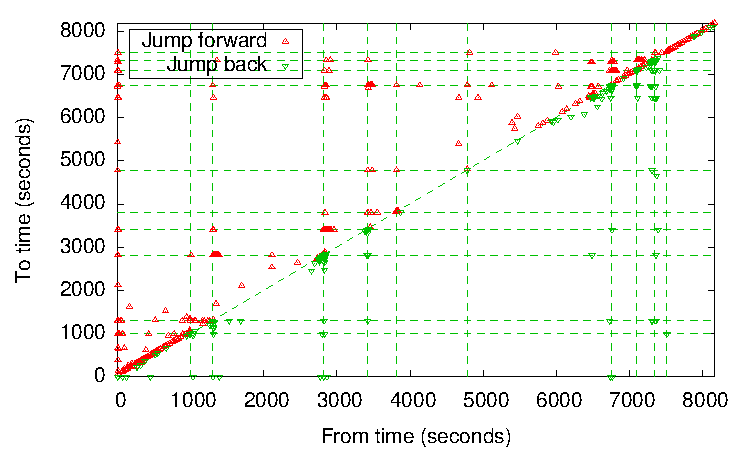
\epsfig{file=./diagrams/arg-scg_jumps.pdf,
width=0.45\textwidth} \caption{\capttext Jumps made by users within
the Argentina vs. Serbia and Montenegro match}
\label{fig:argscg_jumps}
\end{figure}

Vertical and horizontal lines in Fig.~\ref{fig:argscg_jumps}
represent the 10 bookmarks of the match. Every point is a jump that
is identified by corresponding times on both axes.  The diagonal
line is a present-time marker such that the forward jumps are points
which lie above it, while backward jumps appear below it. Thus, no
point falls precisely on the diagonal, yet can be close to it. We
can immediately observe from the figure that many points fall on
horizontal lines, implying that most jumps involved seeking to
bookmarks.

The forward jump buttons appear to have been mostly used for
browsing, as can be seen between 0 and 1000 seconds. This could be
due to user unfamiliarity with the interface, or possibly users
first checking for anything interesting at the start of the video
before moving to a bookmark. The rewind action is used mostly around
events, for example in the case where users wish to re-watch the
event, or when the bookmark insufficiently marked the beginning of
the event. A good example of this was before the bookmark at time
2815, where users rewound up to 75 seconds to see more of the build
up to the goal. Clusters of points can also be seen on horizontal
lines shortly after a vertical line, indicating that users jumped
from one bookmark to another.  We can also observe large clusters
for each vertical line around only one horizontal line, such as from
the bookmark at 1300 seconds going to the bookmark at 2815 seconds.
This shows that a majority of users visited consecutive bookmarks.
In this case users went from the first goal (at time 1300) to the
second goal (at time 2815). The results on this single match
demonstrates that when presented with bookmarks in sports video,
users are highly influenced by them.

\subsection{Popularity}
\begin{figure}[tb]
% ploted with PlotPopularityRank()
\centering 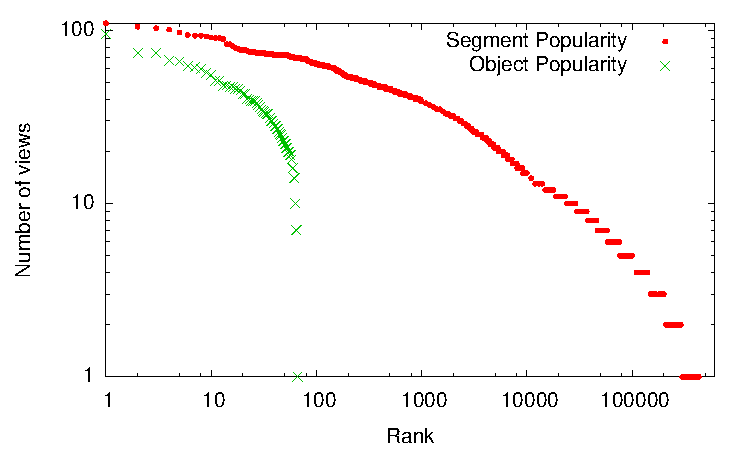
\epsfig{file=./diagrams/all_sessions_rank,
width=0.45\textwidth} \caption{\capttext Object and segment
popularity} \label{fig:popularity_object_rank}
\end{figure}

We study popularity in terms of the number of viewers who watched an
\emph{object} or a \emph{segment}. An object in our system is a
single football match whereas a segment is a section of video one
second in length.

The ranking for both object and segment popularity is shown in
Fig.~\ref{fig:popularity_object_rank}. Recall that there were only
66 matches recorded, which is why the object rank ends much earlier
than for segments. Our analysis reveals that object popularity does
not follow the typical power-law distribution observed within
CDNs~\cite{Chesire01Measurement,Almeida01Analysis,yu2006uub} but
instead is a normal distribution with parameters $\mu = 33.2$ and
$\sigma = 17.1$. This can be attributed to the nature of the World Cup
and the relatively few new objects each day.

\begin{figure}[tb]
\centering 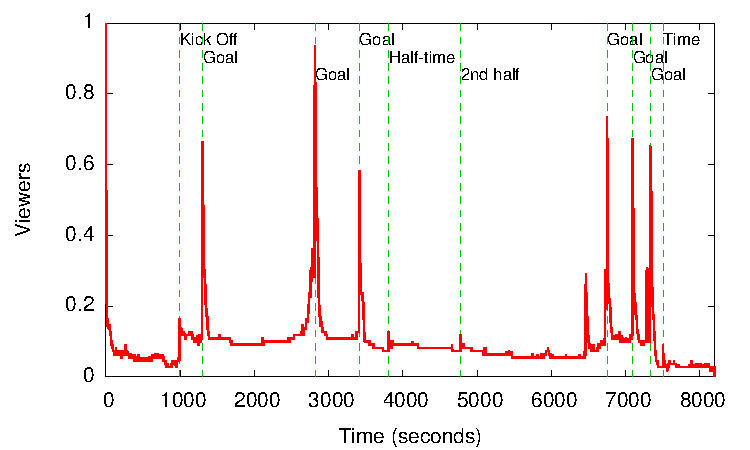
\epsfig{file=./diagrams/arg-scg_views_normal,
width=0.45\textwidth} \caption{\capttext Viewers of the Argentina
vs. Serbia and Montenegro match} \label{fig:arg-scg_views}
\end{figure}

%Pareto R_SQUARE = 0.10983 k = 1.2048
%r_sq=0.094177

We found that the popularity of one-second segments in videos
exhibit a log-normal distribution with parameters $\mu = 0.0159$ and
$\sigma = 1.35$. Note that log-normal distributions closely relate
to power-law or heavy-tailed distributions~\cite{geor06}. They are
skewed distributions where a small percentage of samples contributes
to a sizeable weight of their distribution. We observed that a small
percentage, (the 10\% most popular segments), accounted for about
44\% of all requests. Previously,
Costa~\emph{et~al.}~\cite{Costa04Analyzing} found that for
educational and entertainment content, the popularity of segments is
roughly uniformly distributed with a slight skew towards the
beginning for entertainment content. Our result, however, implies
that there are segments with orders of magnitude more viewers than
others. To illustrate this fact, we present
Fig.~\ref{fig:arg-scg_views}, which shows the popularity of each
second of video for the Argentina vs. Serbia and Montenegro match.
It is very clear from the figure that the bookmarks influence the
popularity of segments. We also observe that most of the bookmarks
that users found interesting are equally popular, receiving requests
from around 60\% of all viewers of the match.

Popularity metrics are important to CDNs as they help to decide what
resources to allocate to each object. We have seen that bookmarked
sports videos provide a content format with specific segments of
interest (goals, for example). This result emphasises the use of
partial caching techniques to cache only popular segments of
objects, as has been previously proposed~\cite{chen2003}.

\subsection{Longevity}
\label{sect:stay_popular}
\begin{figure}[tb]
% plotted with PlotPopularityLifetime()
\centering 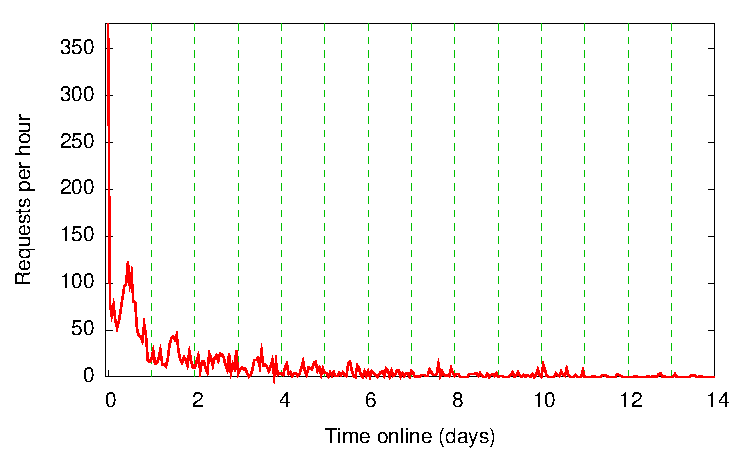
\epsfig{file=./diagrams/all_bookpop_lifetime.pdf,
width=0.45\textwidth} \caption{\capttext Bookmark utilisation over
time, following initial usage} \label{fig:lifetimes}
\end{figure}

The popularity of both videos and bookmarks in our system faded over
time. We call the duration at which any such item remains utilised
its \emph{longevity}. The study of a video or bookmark's longevity
can be used to compute corresponding distributions, aiding in
content management decisions for similar items in the future.

Fig.~\ref{fig:lifetimes} shows the popularity of bookmarks versus
the time they were first utilised. The figure suggests that
following an initial peak and a slight resurgence, there was a rapid
decrease in interest after just a short period.

R-Square fitting reveals that the bookmark longevity can be suitably
estimated using a Weibull distribution with $\lambda=1.814$ and
$k=0.6383$. This suggests that the popularity exhibits heavy-tailed
properties. We also observed that half the bookmark usage occurs
within 24 hours, with the remainder slowly occurring over the
following 2 weeks.

\subsection{Session lengths}
\begin{figure}[tb]
% ploted with PlotSessions2()
\centering 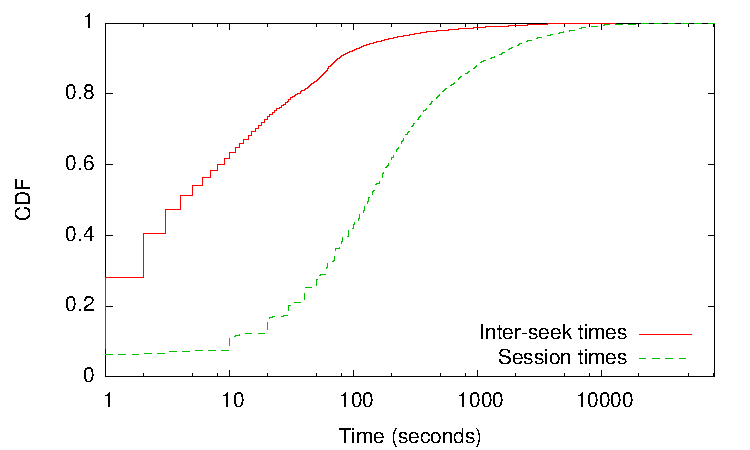
\epsfig{file=./diagrams/view_user_sessions_cdf,
width=0.45\textwidth} \caption{\capttext The CDF of session lengths
and inter-seek times} \label{fig:view_user_session}
\end{figure}

Session length is the total time a user spent on a video. A session
may consist, for example, of a user watching part of a video,
pausing for a while, then continuing to watch the video. Therefore,
it is possible that a session is longer than the actual length of a
video.

Fig.~\ref{fig:view_user_session} shows the CDF of both session and
inter-seek times (discussion on inter-seek times follows in the next
section). It can be observed from the session times that most users
access a video for a very short time relative to the length of the
overall content (\emph{i.e.} possibly just watching interesting
events from the match). In particular, note that around 80\% of
sessions lasted less than 500 seconds. Given that a length of a
typical video was 2.5 hours long, 500 seconds is only 5.5\% of the
video. The average session duration is found to be only 10.2
minutes.

Fig.~\ref{fig:view_user_session} also shows that only a small
minority of users (roughly 3\%) could have possibly watched the
entire match. We found that a small number of users (1.17\%)
accessed the video for between 3 to 8 hours. Our logs show that
these users paused a video for a long time before they decided to
resume playback. These outliers are possibly why we observe that
session sizes are best fitted by a log-normal distribution with
parameters $\mu=4.835$ and $\sigma=1.704$.

\subsection{Inter-seek times}

Inter-seek time is described as the time a user spent actually
watching a section of a video before seeking to a new location
(disregarding any paused periods within the session).

From our logs, we found that on average a user performed 9.3 seek
operations around a video resulting to a mean inter-seek time of 66
seconds. Fig.~\ref{fig:view_user_session} shows the CDF for
inter-seek times as well as session length. It can be seen that the
majority of users viewed the content as a series of excerpts,
usually under a minute in length.

%It can been seen that around 50\% of viewed sections of videos were
%less than 8 seconds in length, and around 80\% of users watched the
%video for less than 50 seconds before seeking again. Less than 1\%
%of all users watched more than 1000 seconds of consecutive video.

We found that inter-seek times can be estimated by a log-normal
distribution with parameters $\mu=1.4796$ and $\sigma=2.2893$.
Previous studies have also found that the majority of inter-seek
times are very short~\cite{vilas2005user}. They have also been shown
to be approximately {\em Poisson} or {\em Pareto} for educational
content in different servers~\cite{Almeida01Analysis}. A
distribution of inter-seek times can be used by a delivery system to
determine the size of video replicas and the time that it should
react before a user seeks elsewhere on the video.

\subsection{Sequence}
\begin{figure}[tb]
%plotted with PlotSequence()
\centering 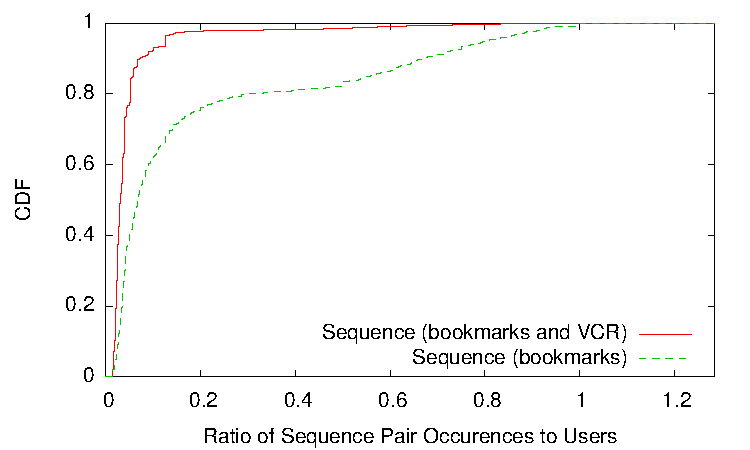
\epsfig{file=./diagrams/all_sequence_normal_cdf,
width=0.45\textwidth} \caption{\capttext The ratio of sequence pairs
to the number of users that watched them} \label{fig:all_sequence}
\end{figure}

In this section, we analyse the data we collected from our
experiment to study the extent to which user actions on a video can
be predicted. We call the order that events in a single match are
viewed a {\em sequence} of events. A typical sequence can include
any combination of user actions on a video such as starting the
video, VCR actions, seeking to a bookmark, \emph{etc}. Additionally,
we separately consider sequences that consist of jumping between
bookmarks. If a system could detect or predict patterns within a
sequence, then it could pro-actively respond to them in order to
optimise content delivery. For example, a server could use spare
bandwidth to push out the appropriate content to a user before being
requested, or a client could be allowed to pre-cache content based
on popularity of a pattern in a sequence.

We first identified sequences of actions from our traces. We then
broke the sequences into pairs of events that were accessed
consecutively. For example, a sequence made up of starting the
video, jumping from bookmark $A$ to bookmark $B$, forwarding 30
seconds (F30), and finally ending a session was broken into 4 pairs,
namely, $Start \rightarrow A$, $A \rightarrow B$, $B \rightarrow
F30$, $F30 \rightarrow End$. Note that the event {\em End} means the
end of a session and not necessarily the end of a video. The number
of occurrences of each pair was totalled for each match and
normalised by the number of users who watched that match. The ratio
of users to each sequence pair is shown as a CDF (for both bookmarks
alone and inclusive of VCR actions) in Fig.~\ref{fig:all_sequence}.
Note that the x-axis of the figure goes above 1, which shows that
some sequence pairs have been followed more than once by some users.
Intuitively, the more the sequence pair is followed, the more
predictable it is, and thus larger values on the x-axis represent
better predictability for a given sequence.

Fig.~\ref{fig:all_sequence} shows that around the top 20\% of
bookmark sequence pairs were followed by more than 50\% of users.
This means that there is a high chance of predicting these bookmark
sequences. Note that these bookmarks also consist of the 20\% most
popular bookmarks. However, the figure also shows that it is
generally difficult to predict the actions of a user if all actions
are considered. This is because of the wider range of interactivity
options a user has when VCR functionality is also considered.

\begin{table}[tb]
\centering {\tiny
\begin{tabular}{|c|c|c|}
  \hline
  Metric & Distribution & R-square \\
  \hline
  Object Popularity  & Normal, $\mu=33.20$ , $\sigma=17.10$      & 0.0260 \\
  Segment Popularity & Log-normal, $\mu=0.016$ , $\sigma=1.35$   & 0.0941 \\
  Session size       & Log-normal, $\mu=4.835$, $\sigma=1.704$   & 0.127  \\
  Inter-seek times   & Log-normal, $\mu=1.4796$, $\sigma=2.2893$ & 0.0358 \\
  %Game Longevity     & Weibull, $\lambda=2330$ , $k=0.664$       & 0.163  \\
  Bookmark Longevity & Weibull, $\lambda=1.814$ , $k=0.6383$     & 0.0372 \\
\hline
\end{tabular}}
\caption{\capttext A summary of metrics with their corresponding
distributions} \label{tab.summary}
\end{table}

We now summarise the analytical models in Table~\ref{tab.summary}.
We found that user metrics could be estimated by more than one
distribution, however the table shows only the best fit for each.
The table also shows corresponding {\em R-square} values that illustrate
the suitability of the models. Of particular importance is the type of
distribution which can have a significant impact on the system. For example,
the Weibull and log-normal distributions are both heavy-tailed, for which
systems may have to anticipate the uneven distribution to cope effectively.

%The exact parameters are of little importance, however the type of distribution used implies the impact on the system.

%Observe that
%the {\em log-normal} distribution emerges as the best model for most
%of the observed features in our experiment, except for object
%popularity and arrival rates, which are best modelled by {\em Normal
%} and {\em Weibull} distributions respectively. This is unsurprising
%because log-normal distributions are commonly known to model various
%properties in computing systems. Weibull and, as noted earlier,
%log-normal distributions both closely relate to power-law or
%heavy-tailed distributions~\cite{geor06}.

\section{Conclusions and Future Work}
\label{sect:conclusion}

We have presented a study and characterisation of user behaviour for
interactive sports video-on-demand (VoD) systems. Using our
custom-built VoD system, we captured FIFA 2006 World Cup matches and
made them locally available through a highly interactive user
interface.

Our results show that the interactivity options available to users
highly influence their behaviour. In particular, we found that the
novel interactive feature called {\em bookmarking}, played a pivotal
role, leading to access patterns quite dissimilar from previous
related studies that looked at VCR-like interactivity alone. The
combination of our content type and the addition of bookmarks led to
users accessing content in relatively small segments that were both
highly popular and sparsely distributed throughout the length of the
videos. These popular segments, more commonly named hotspots, were clearly skewed
around bookmarks. From both a user and a CDN's perspective, this
can be viewed as advantageous; users can reach interesting content
more quickly through the bookmarks, and the increased locality of
interest means the CDN can respond more effectively.

%\section{Future work}
%\label{sect:future_work}

Interest in a given event is subjective, however, and an
administrator or individual user's opinion inevitably plays a major
part in the optimality of manually placed bookmarks in terms of
their locations and validity. For delivery networks to benefit from
the user characterisation observed in this paper, it is clear that
they must be optimised to allow for autonomic repositioning of
incorrectly placed bookmarks, detection of hotspots, and
caching/replication, all based on predicted or past recorded user
behaviour.

% \subsection{Autonomic Hotspot Detection}

A particular section of a piece of content may prove to be far more
popular than the remainder, thus making it suitable for special
treatment. Service providers can either rely on their users or
administrators to add appropriate metadata describing potential
hotspots on the video. However, neither would necessarily know how
demand for their content would change over time. As such, reactive
and adaptive approaches may prove most suitable for the general
case, where the evolution of hotspots and the validity of bookmarks
are autonomically detected based on observed patterns.

A simple way of achieving this would be to select a threshold
(\emph{e.g.} a percentage of users) and classify any section of
video which exceeds it as a hotspot. This method may take time to
identify the correct hotspots since requests must first be recorded
across the length of a video. The system could then mark an
identified hotspot with a bookmark for easy access to future users.
Additionally, longevity information can be used in conjunction with
detection algorithms to decide upon the validity of existing
bookmarks.

% \subsection{Bookmark repositioning}

\begin{figure}[tb]
%plotted with PlotBacks()
\centering 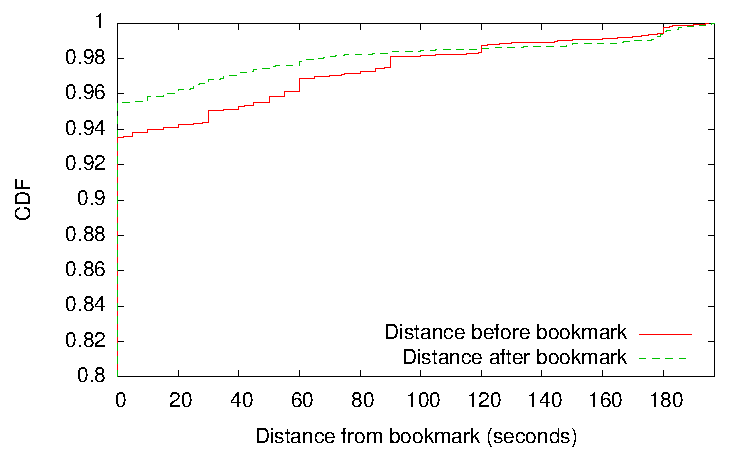
\epsfig{file=./diagrams/all_backs_cdf-20.pdf,
width=0.45\textwidth} \caption{\capttext Difference between bookmark
start and maximum sought distance} \label{fig:bookmark_rewind_diffs}
\end{figure}

Upon examination of our logs, we found that some of the bookmarks
were incorrectly placed. Users who discovered that the bookmark
started sooner or later than they expected are likely to make a
corresponding jump shortly after requesting a bookmark (as observed
in Fig.~\ref{fig:argscg_jumps}). We observed that 40\% of the
bookmarks had at least one user who jumped to a position before the
bookmark itself. Upon inspection of the video content, however, we
discovered that when users consistently made an additional seek, it
was typically because bookmarks were placed during the run-up to a
penalty kick, omitting the cause of it. Users wanting to see the
relevant incident would therefore have to seek backwards, as the
bookmarks were incorrectly placed beyond the beginning of the actual
hotspot.

We also analysed the distance from a bookmark that users jumped
shortly after requesting it (within a range of 200 seconds either
side, as to ensure relevancy to the bookmark). An examination of the
traces revealed that approximately 84\% of the seeks considered were
carried out within 20 seconds of moving to the bookmarks, perhaps
representing the users who were almost immediately dissatisfied with
the bookmark location. Fig~\ref{fig:bookmark_rewind_diffs} shows the
varying distances from the bookmark that users moved to, all within
20 seconds of reaching the bookmark's location. We observe from the
figure that around 6\% of bookmark requests have seeks shortly
afterwards, possibly due to suboptimal bookmark positioning. It was
noted that 5.7\% of all bookmark requests were for penalties, adding
support to this theory.

Placing bookmarks optimally has the advantage of improving user
experienced performance and reducing load on servers, whereas
incorrectly positioning bookmarks leads to an increase in the number of
seeking requests. It is therefore desirable for a delivery system to
be capable of repositioning relevant bookmarks accordingly to enable
faster access of relevant content, and the resultant reduction in
seek operations would reduce network load.

We experimented with a repositioning mechanism based on a
exponentially-weighted moving average algorithm, using our logs as
input. We observed that the algorithm successfully identified the
correct positions for poorly positioned bookmarks and left the
positions of well positioned bookmarks unchanged (results are
omitted due to lack of space). In our future work, we will check to
see if such an algorithm can perform similarly in delivery networks
and we will devise new algorithms if necessary.

% \subsection{Caching Strategies}

Beyond issues related to their placement, the resultant effect of
bookmarking was that several sections of each video were far more
popular than others. In a CDN context, this reaffirms the idea that
content should not be treated as immutable objects, and instead it
should be divided into small segments. A network can then rank the
segments in terms of their popularity and apply caching or
replication strategies accordingly.

Naturally, the size of the segments in question is an important
concern. In this paper we have examined the content on a
second-by-second basis; while this may seem a small value given that
all our videos were several hours long,
Fig.~\ref{fig:view_user_session} indicates that 60\% of all
sustained playback operations were actually 10 seconds or less, and
thus small segment sizes would potentially be required.

Developing algorithms to predict the actions of newly arriving users
based on the experience of past users may also prove useful. For
example a CDN could infer the order of segments users typically
viewed, or the probability of viewing any given segment after
another. This could form a probability matrix with each destination
weighted by the percentage of previous users who chose that
destination; knowledge which may then be useful to both the server
and the client. On the server side, the server would be aware of
which content to {\em pre-fetch} from the original source or {\em
pre-push} to other servers or clients in advance. This could also
influence {\em caching eviction} decisions whereby objects are
evicted based on their usage as well as the popularity of objects
likely to be requested with them.

Future work may involve expansion upon all of these concepts, along
with further characterisation of differing content types.

\bibliographystyle{abbrv}
\bibliography{worldcup}

\end{document}
